\section{Problem 3}
\label{part3}
\subsection*{Question}
\begingroup
\begin{verbatim}

3. Download and install Gephi:

https://gephi.org/

Load the dot file created in #2 and use Gephi to:

- visualize the graph (you'll have to turn on labels)
- calculate HITS and PageRank
- avg degree
- network diameter
- connected components

Put the resulting graphs in your report.

You might need to choose the 100 sites with an eye toward
creating a graph with at least one component that is nicely
connected.  You can probably do this by selecting some portion
of your links (e.g., 25, 50) from the same site.  

\end{verbatim}
\subsection{Answer}

\begin{enumerate}
\item The graph described by the dot file in Question 2 contain 3021 nodes and 3176 edges. 
\item From Gephi, visualizing the graph produced an unclear graph shown in Figure \ref{fig:q3-1}
\item So I used Yifan Hu Proportional layout, the graph became much better as shown in Figure \ref{fig:q3-2}. This graph is with out labels. 
\item After that I enabled the labels for the Figure \ref{fig:q3-2} which resulted as Figure \ref{fig:q3-3}
\item I saved the Figure \ref{fig:q3-1} , \ref{fig:q3-2} and \ref{fig:q3-3} in pdf format from Gephi so that we can see the labels clearly if image is zoomed.
\item Figure \ref{fig:q3-4} shows low authority scores on all pages. Figure \ref{fig:q3-5} shows what look to be two hubs. 
\item PageRank for all pages approaches 0 as shown in Figure \ref{fig:q3-6} because so many pages link to one another. 
\item Figure \ref{fig:q3-8} shows that very few nodes have in-degree values. 
Surprisingly Figure \ref{fig:q3-9} shows that a lot of pages do seem to link out but in an almost horizontal linear pattern. 
\item The graph has a network diameter of 1 , with 3173 shortest paths. The average path length is 1.0. 
\item Figure \ref{fig:q3-11} shows most of the nodes are so connected that their closeness is quite low.
\item Figure \ref{fig:q3-13} shows that 3201 components are strongly connected in this graph. And 58 components are weakly connected.
\end{enumerate}

\begin{figure}
	 \begin{center}
		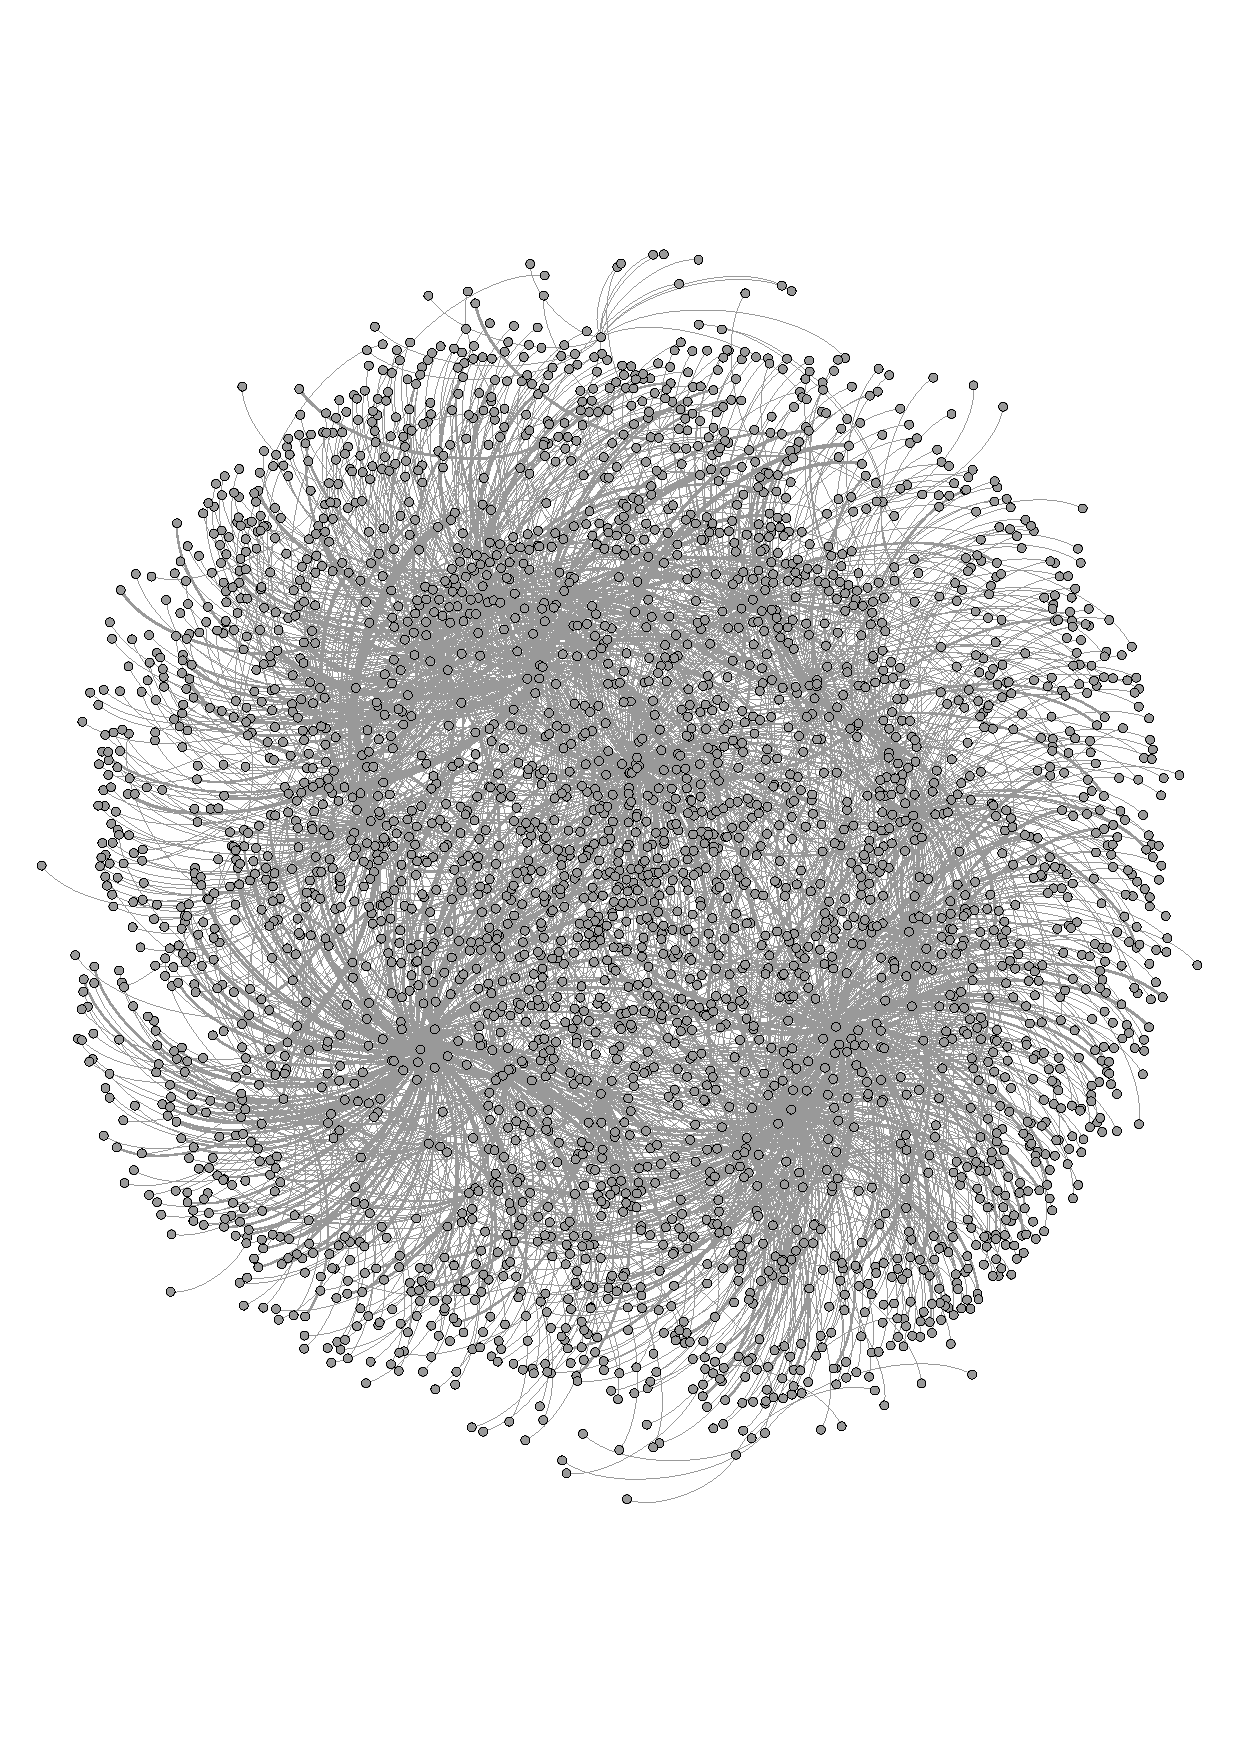
\includegraphics[scale=0.8]{q3/a4-q3-1.pdf}
		\caption{Initial Visualization of the graph for DOT file from Question 2}
		\label{fig:q3-1}
 	\end{center}
\end{figure}

\begin{figure}
	 \begin{center}
		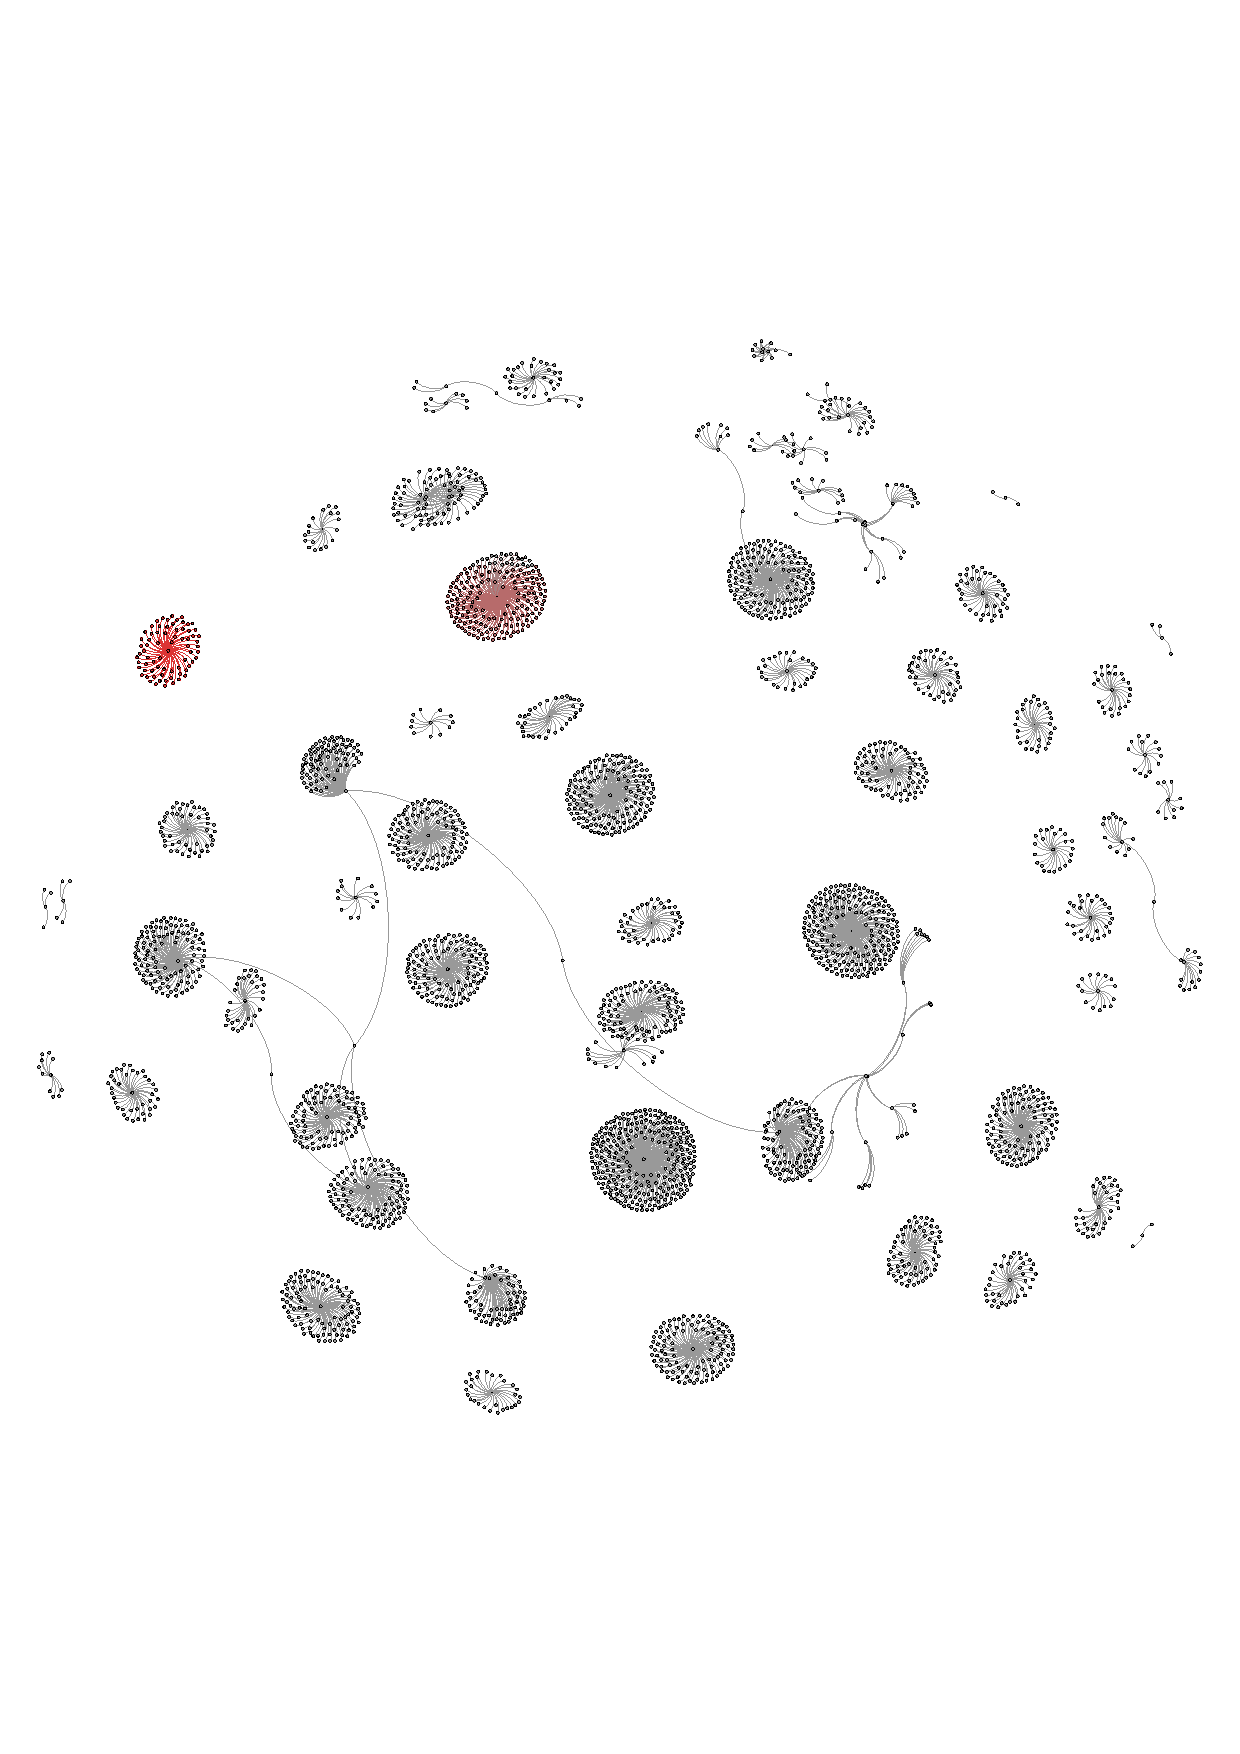
\includegraphics[scale=0.8]{q3/A4_q3_without_labels.pdf}
		\caption{Graph with Yifan Hu layout}
		\label{fig:q3-2}
 	\end{center}
\end{figure}
\subsubsection{Graph with Yifan Hu layout with labels}
\begin{figure}
	 \begin{center}
		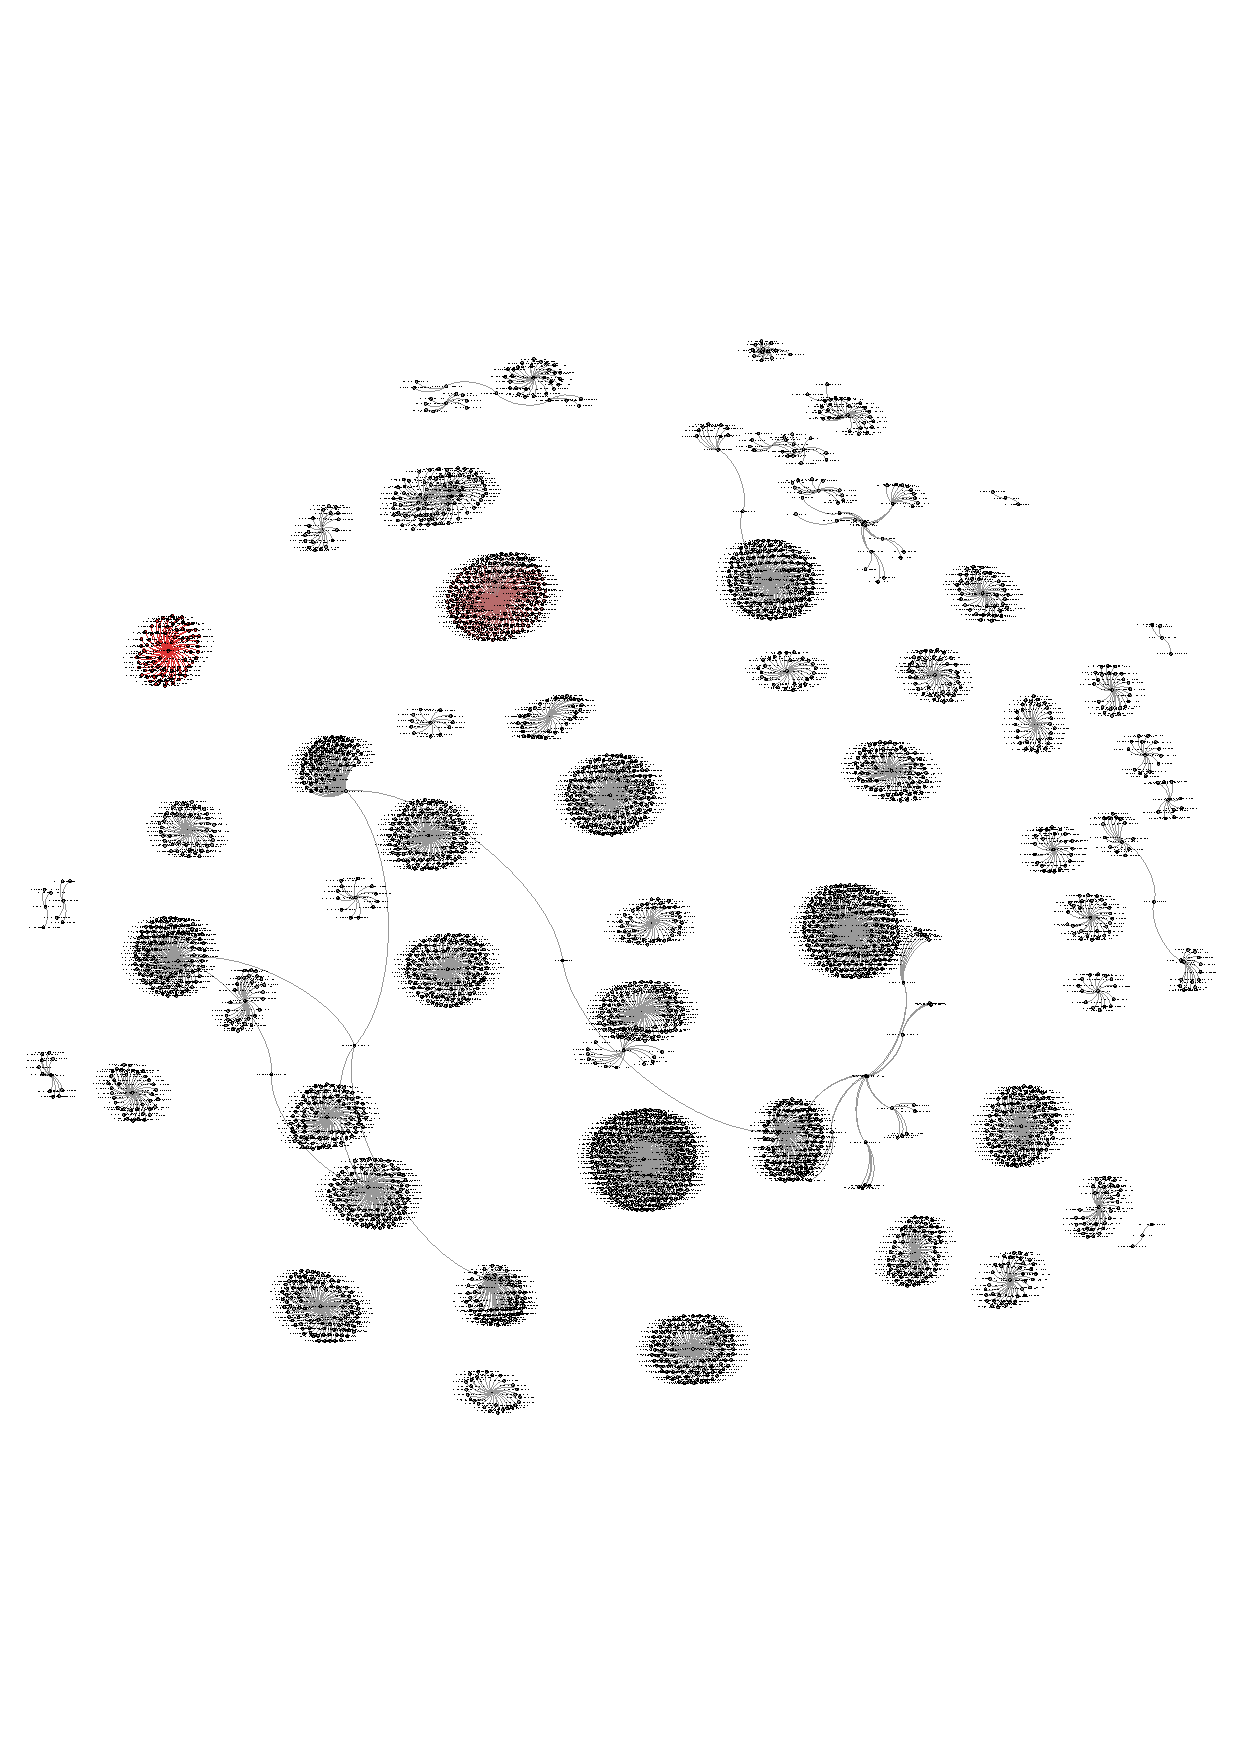
\includegraphics[scale=0.8]{q3/A4_q3_with_labels.pdf}
		\caption{Graph with Yifan Hu layout with labels}
		\label{fig:q3-3}
 	\end{center}
\end{figure}
\newpage
\subsubsection{HITS and PageRank}
\begin{figure}[!ht]    
    \begin{center}
        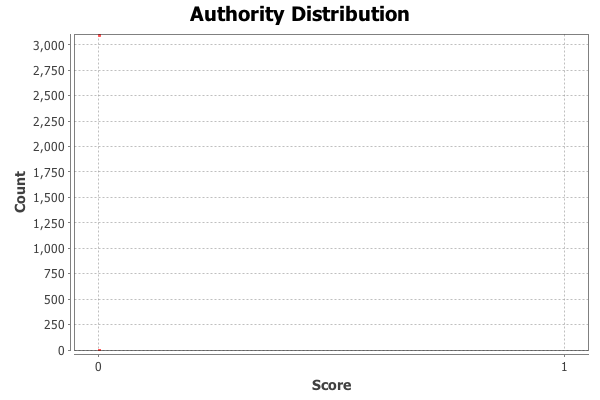
\includegraphics[scale=0.60]{q3/HITS/authorities.png}
        \caption{Authority Distribution for HITS}
        \label{fig:q3-4}
    \end{center}
\end{figure}
\begin{figure}[!ht]    
    \begin{center}
        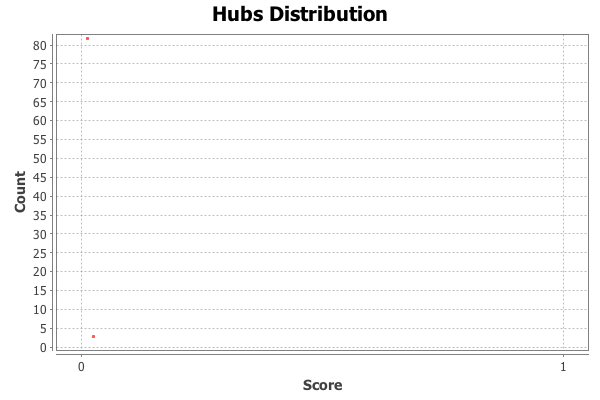
\includegraphics[scale=0.60]{q3/HITS/hubs.png}
        \caption{Authority Distribution for HITS}
        \label{fig:q3-5}
    \end{center}
\end{figure}
\begin{figure}[!ht]    
    \begin{center}
        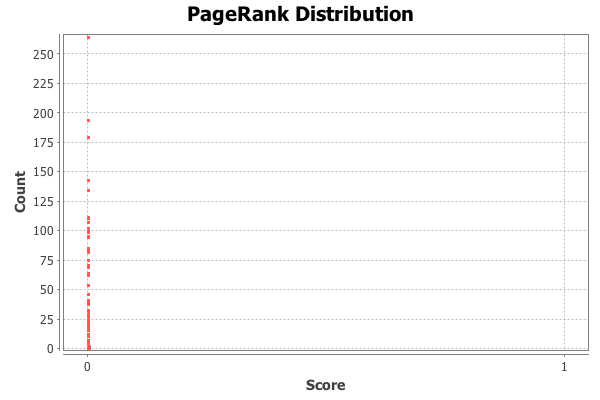
\includegraphics[scale=0.60]{q3/PageRank/pageranks.png}
        \caption{PageRank Distribution for PageRanks}
        \label{fig:q3-6}
    \end{center}
\end{figure}
\newpage

\begin{figure}[!ht]    
    \begin{center}
        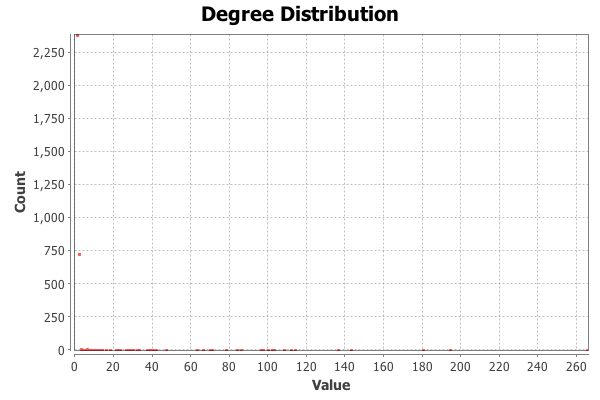
\includegraphics[scale=0.60]{q3/AverageDegree/degree-distribution.png}
        \caption{Degree Distribution for Average 
        degree}
        \label{fig:q3-7}
    \end{center}
\end{figure}
\begin{figure}[!ht]    
    \begin{center}
        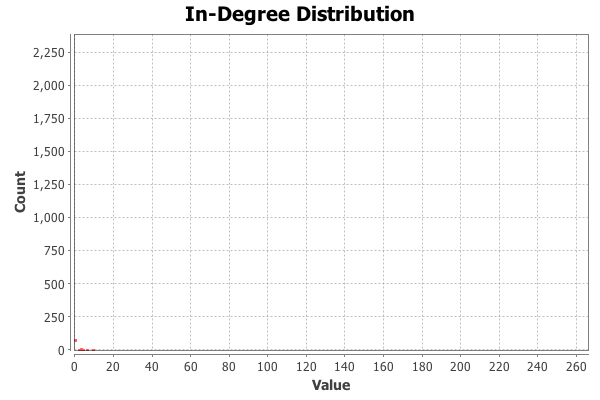
\includegraphics[scale=0.60]{q3/AverageDegree/indegree-distribution.png}
        \caption{In-Degree Distribution for Average 
        degree}
        \label{fig:q3-8}
    \end{center}
\end{figure}
\begin{figure}[ht]    
    \begin{center}
        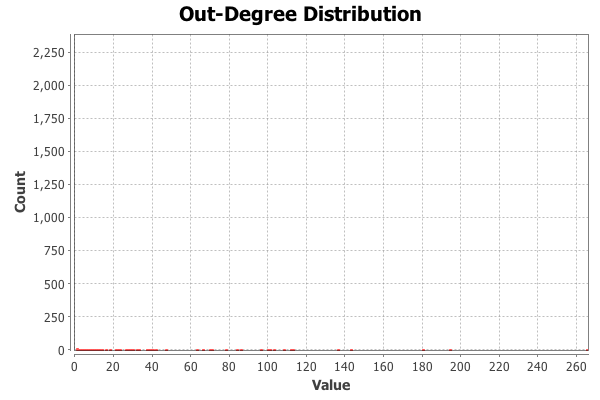
\includegraphics[scale=0.60]{q3/AverageDegree/outdegree-distribution.png}
        \caption{Out-Degree Distribution for Average 
        degree}
        \label{fig:q3-9}
    \end{center}
\end{figure}
\newpage

\begin{figure}[!ht]    
    \begin{center}
        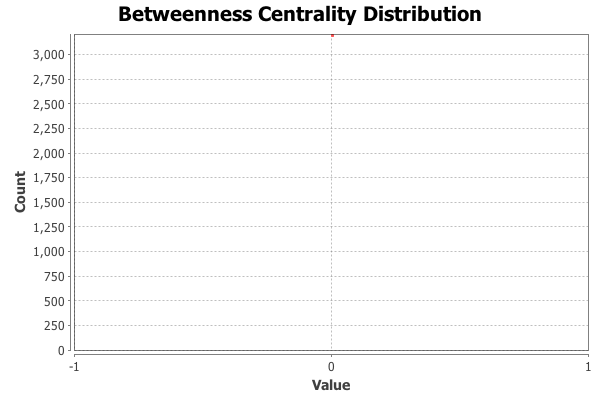
\includegraphics[scale=0.60]{q3/NetworkDiameter/BetweennessCentralityDistribution.png}
        \caption{Betweenness Centrality Distribution for Network Diameter}
        \label{fig:q3-10}
    \end{center}
\end{figure}
\begin{figure}[!ht]    
    \begin{center}
        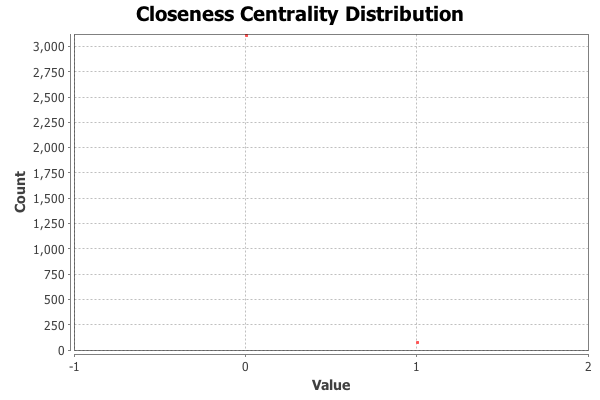
\includegraphics[scale=0.60]{q3/NetworkDiameter/ClosenessCentralityDistribution.png}
        \caption{Closeness Centrality Distribution for Network Diameter}
        \label{fig:q3-11}
    \end{center}
\end{figure}
\begin{figure}[ht]    
    \begin{center}
        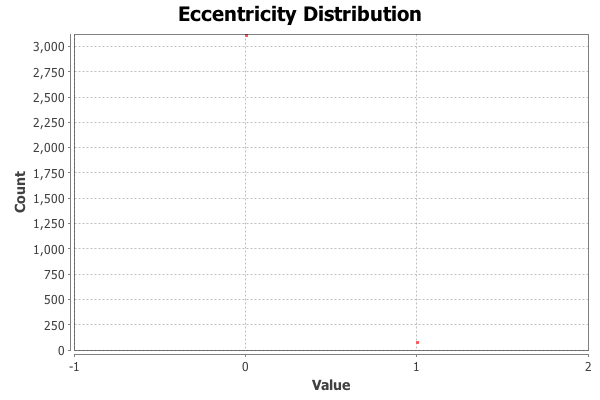
\includegraphics[scale=0.60]{q3/NetworkDiameter/EccentricityDistribution.png}
        \caption{Eccentricity Distribution for Network Diameter}
        \label{fig:q3-12}
    \end{center}
\end{figure}
\newpage


\begin{figure}[ht]    
    \begin{center}
        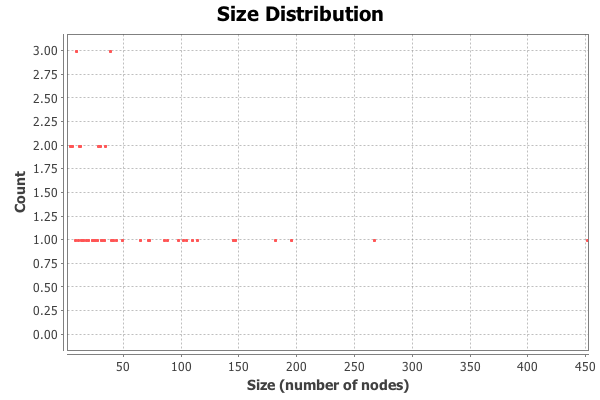
\includegraphics[scale=0.60]{q3/ConnectedComponents/ccSizeDistribution.png}
        \caption{Size Distribution for Connected Components}
        \label{fig:q3-13}
    \end{center}
\end{figure}

